\chapter{Цуваа} \index{Цуваа}
\section{Тоон цуваа}
Гишүүд нь комплекс $z_k=x_k+iy_k$ тоо байх
\begin{eqnarray} \label{5.1}
   z_1+z_2+\cdots +z_k+\cdots =\sum\limits_{k=1}^\infty z_k
\end{eqnarray}
цуваа авч үзье.

Бодит гишүүдтэй цувааных шиг
\begin{eqnarray}
   S_n=\sum\limits_{k=1}^n z_k
\end{eqnarray}
тоог цувааны хэсгийн нийлбэр гэнэ. Хэрэв хэсгийн нийлбэрийн хязгаар $S=\lim\limits_{n\rightarrow \infty} S_n$ оршин байвал (\ref{5.1}) цувааг нийлэх гэх ба $S$ тоог уул цувааны нийлбэр гэнэ. Өөрөөр хэлбэл $S=\sum\limits_{k=1}^\infty z_k$ гэнэ. Хэсгийн нийлбэрт төгсгөлтэй хязгаар оршин байхгүй бол (\ref{5.1}) цувааг сарних гэнэ.

Нийлэх цувааны ерөнхий $z_n$ гишүүн тэг рүү тэмүүлнэ. Учир нь (\ref{5.1}) нийлэх цуваа гэвэл

$$\lim\limits_{n\rightarrow \infty}z_n=\lim\limits_{n\rightarrow \infty} (S_n-S_{n-1})=S-S=0$$
Үүнийг цувааны нийлэлтийн зайлшгүй нөхцөл гэнэ. (\ref{5.1}) цувааны нийлэхийн зайлшгүй бөгөөд хүрэлцээтэй нөхцөл нь $\sum\limits_{k=1}^\infty x_k$ ба $\sum\limits_{k=1}^\infty y_k$-цуваануудын нийлэх явдал мөн. Иймд $\sum\limits_{k=1}^\infty z_k=S$, $\sum\limits_{k=1}^\infty x_k=\alpha$, $\sum\limits_{k=1}^\infty y_k=\beta$ гэвэл $S=\alpha +i\beta$ 
байна.
\begin{thm}
\textbf{(Нийлэлтийн Кошийн шинжүүр) } \index{Кошийн шинжүүр} (\ref{5.1}) цуваа нийлэх зайлшгүй бөгөөд хүрэлцээтэй нөхцөл нь аливаа $\varepsilon >0$ тооны хувьд натурал $N=N(\varepsilon)$ олдож $n>N$ ба ямар ч натурал $p$ тооны хувьд
\begin{eqnarray}
   |S_{n+p}-S_n|=|z_{n+1}+z_{n+2}+\cdots +z_{n+p}|=\left|\sum_{k=n+1}^{n+p}z_k\right| <\varepsilon
\end{eqnarray}
биелэгдэх явдал мөн. (\ref{5.1}) цувааны гишүүдийн модулиудаас зохиосон
\begin{equation} \label{5.4}
    \sum\limits_{k=1}^\infty |z_k|
\end{equation}
цуваа нийлж байвал (\ref{5.1}) цуваа нийлнэ.

Энэ нь Кошийн шинжүүрээр нотлогдоно:
$$\left|\sum_{k=n+1}^{n+p}z_k\right|\leq \sum_{k=n+1}^{n+p}|z_k|.$$
Энэ үед (\ref{5.1}) цувааг абсолют нийлэлттэй цуваа гэнэ. Харин (\ref{5.4}) цуваа сарниж байхад (\ref{5.1}) цуваа нийлэх тохиолдол байдаг. Энэ үед (\ref{5.1}) цувааг нөхцөлт нийлэлттэй цуваа гэнэ.

Цувааны абсолют нийлэлт тогтоохын тулд эерэг гишүүдтэй бодит цувааны нийлэлтийн хүрэлцээт шинжүүдийг ашиглана. Дэлгэр хэрэглэгддэг зарим шинжүүдийг баталгаагүйгээр тэмдэглэе:
\end{thm} 
\textbf{Жишилтийн шинж.} $\forall k>N$-ийн хувьд $|z_k|\leq |w_k|$ байхад $\sum\limits_{k=1}^\infty |w_k|$ цуваа нийлэх бол $\sum\limits_{k=1}^\infty |z_k|$ цуваа нийлнэ.\\
\textbf{Даламберийн шинж.} $\forall k>N$-ийн хувьд $\dfrac{|z_{k+1}|}{|z_k|}\leq q<1$ байвал (\ref{5.4}) цуваа нийлнэ. Харин $\forall k>N$-ийн хувьд $\dfrac{|z_{k+1}|}{|z_k|}\geq 1$  байвал (\ref{5.4}) цуваа сарнина. \\
\textbf{Кошийн шинж.} $\forall k>N$-ийн хувьд $\sqrt[k]{|z_k|}\leq q<1$ байвал (\ref{5.4}) цуваа нийлнэ. Харин $\forall k>N$-ийн хувьд $\sqrt[k]{|z_k|}\geq 1$ байвал (\ref{5.4}) цуваа сарнина.
\section{Функцэн цуваа} \index{Функцэн цуваа}
$f_k(z)\in H(D)$ функцүүдээс зохиосон
\begin{eqnarray} \label{5.5}
   \sum\limits_{k=1}^\infty f_k(z)
\end{eqnarray}
дүрсийн цуваа авч үзье. Энэ цувааны нийлэх $z\in D$ цэгүүдийн олонлогийг түүний нийлэлтийн муж гэнэ. 

Нийлэлтийн энэ муж дээр (\ref{5.5}) цувааны нийлбэр
$$S(z)=\sum\limits_{k=1}^\infty f_k(z)$$
ба түүний үлдэгдэл
$$r_n(z)=S(z)-S_n(z)=\sum\limits_{k=n+1}^\infty f_k(z)$$
гэж тодорхойлогдсон байг. (\ref{5.5}) цуваа ямар нэг $G$ муж дээр $S(z)$ рүү нийлдэг байг. Функцэн цувааны хувьд жигд нийлэлтийн асуудлыг чухалчилдаг.
\begin{dfn}
 Функцэн (\ref{5.5}) цуваа $\forall \varepsilon>0$-ийн хувьд зөвхөн $\varepsilon$ тооноос хамааран $N=N(\varepsilon)$ дугаар олдож $N<n$ байх бүх $n$-ийн үед $G$ муж дээр
 $$|S(z)-S_n(z)|=|r_n (z)|<\varepsilon$$
нөхцөл $(S_n(z)=  \sum\limits_{k=1}^n f_k(z)$- хэсгийн нийлбэр) биелэгдэж байвал  функцэн (\ref{5.5}) цуваа $G$ муж дээр жигд нийлж байна гэдэг.
\end{dfn}
Нийлэх функцэн цуваа бүр жигд нийлэх нь албагүй.

Жишээ нь хэсгийн нийлбэр нь
$$S_n(z)=\sum\limits_{k=0}^n z^n=\frac{1-z^{n+1}}{1-z}$$
байх
$$\sum\limits_{k=0}^n z^k$$
геометр прогресс нэгж $|z|<1$ дугуй дээр $S(z)=\dfrac{1}{1-z}$ рүү абсолют нийлнэ. Учир нь
$$\lim\limits_{n\rightarrow \infty} S_n(z)=\lim\limits_{n\rightarrow \infty} \frac{1-z^{n+1}}{1-z}=\frac{1}{1-z}\qquad |z|<1.$$
Гэтэл энэ цуваа $|z|<1$ дээр жигд биш нийлнэ. Учир нь үлдэгдэл гишүүн нь $\dfrac{1}{2}<|z|<1$ үед доороосоо
$$|r_n (z)|=\dfrac{|z|^{n+1}}{|1-z|}\geq \frac{|z|^{n+1}}{1-|z|}\geq \frac{1}{2^{n+1}(1-|z|)}$$
гэж үнэлэгдэнэ.

Иймд дурын бэхлэгдсэн хүрэлцээт их $n$-авахад $|z|$-ийг нэгжид хүрэлцээтэй ойр сонгох замаар үлдэгдлийн модулийг урьдчилан өгөгдсөн ямар ч тооноос ихээр авах боломж олдоно.

\begin{thm}
\textbf{(Жигд нийлэлтийн Вейерштрассын шинжүүр). } \index{Жигд нийлэлтийн Вейерштрассын шинжүүр}(\ref{5.5}) цувааны $k$ тооны гишүүдийн хувьд $G$ муж дээр $|f_k(z)|\leq c_k(k=1,2,3,\ldots)$ тэнцэл биш биелэгдэхэд $\sum\limits_{k=1}^\infty c_k$ нь  нийлэх тоон цуваа (мажорант цуваа) байвал уул функцэн цуваа $G$ муж дээр абсолют бөгөөд жигд нийлнэ.
\end{thm}
\begin{prf}
Абсолют нийлэх нь жишилтийн шинжээр шууд тогтоогдоно. Цааш нь (\ref{5.5}) цувааны нийлбэр ба хэсгийн нийлбэрийг харгалзан $S(z)$, $S_n(z)$ гэж тэмдэглэвэл 
$$|S(z)-S_n(z)|\leq \sum\limits_{k=n+1}^\infty |f_{k}(z)|\leq \sum\limits_{k=n+1}^\infty c_k$$
бөгөөд аливаа $\varepsilon >0$ авахад $N=N(\varepsilon)$ дугаар олдож $n\geq N$ байх $n$-ийн хувьд $\sum\limits_{k=n+1}^\infty c_k<\varepsilon$ болж теорем батлагдав. 
\end{prf}
\begin{thm} \label{Теорем 2}
$f_n(z)=H(G)$ байг. (\ref{5.5}) цуваа $G$ дээр жигд нийлж байвал $S(z)$ нийлбэр нь $G$ дээр тасралтгүй байна.
\end{thm}
\begin{prf}
$\varepsilon >0$ ба $z_0\in G$ өгөгдсөн байг. Цувааны хэсгийн нийлбэрийн хувьд $|S(z)-S_n(z)|<\dfrac{\varepsilon}{3}$ тэнцэл биш биелэгдэж байхуйц $n$ тоо сонгон авъя. $S_n(z)$ нийлбэр $G$ дээр тасралтгүй тул $|z-z_0|<\delta$ байвал $|S_n(z)-S_n(z_0)|<\dfrac{\varepsilon}{3}$ байхаар $\delta > 0$ олдоно.

Одоо $S(z)-S(z_0)$ ялгаврын хувьд
\begin{align*}
    |S(z)-S(z_0)|&=|S(z)-S_n(z)+S_n(z)- \\
    &-S_n(z_0)+S_n(z_0)-S(z_0)|<\frac{\varepsilon}{3}+\frac{\varepsilon}{3}+\frac{\varepsilon}{3}=\varepsilon
\end{align*}
болж теорем батлагдав.
\end{prf}
Энэ теорем $f_n(z)$ нь $G$ дээр зөвхөн тасралтгүй байх тохиолдолд ч үнэн байна.

Функцүүдийн төгсгөлтэй нийлбэрийг гишүүнчлэн интегралчилж болдгийг бид интеграл тооллоос мэднэ. Харин цувааг гишүүнчлэн интегралчлах нь өвөрмөц нөхцөлөөр шийдэгдэхийг дараах теоремоос танилцъя.
\begin{thm}
$\Gamma \subset G$ шугам дээр тасралтгүй функцүүдийн жигд нийлэх цувааг гишүүнчлэн интегралчлана: 
\begin{eqnarray}
   \int\limits_{\Gamma} S(z)dz=\sum\limits _{k=1}^\infty \int\limits_{\Gamma} f_k(z)dz
\end{eqnarray}
\end{thm}
\begin{prf}
$S(z)=\sum\limits_{k=1}^\infty f_k(z)$ байг. $\displaystyle\int\limits_{\Gamma} S(z)dz$ оршин байна. Учир нь $S(z)$ функц $\Gamma$ дээр тасралтгүй (өмнөх Теорем 5.3) интегралчлагдсан цувааны хэсгийн нийлбэр $\sigma_n$ гэвэл
$$\sigma_n= \sum\limits_{k=1}^n\int\limits_{\Gamma} f_k(z)dz=\int\limits_\Gamma S_n(z)dz$$
бөгөөд одоо
\begin{eqnarray} \label{5.7}
   \lim\limits_{n\rightarrow \infty} \sigma_n =\int\limits_\Gamma S(z)dz
\end{eqnarray}
гэж батлах хэрэгтэй.

$\varepsilon > 0$ байг. Энэ тохиолдолд теоремын нөхцөл ёсоор $N$ тоо авахад $n>N$ үед $|S(z)-S_n(z)|<\varepsilon$ байна. Тийм $n$-ийн хувьд 
\begin{align*}
    \left|\int\limits_{\Gamma} S(z)dz-\sigma _n \right|&= \left|\int\limits_{\Gamma} [S(z)-S_n(z)]dz\right|\leq \\
    &\leq \int\limits_{\Gamma}|S(z)-S_n(z)|\cdot |dz|<\varepsilon l.
\end{align*}
Үүнд $I$ нь $\Gamma$ шугамын урт. Эндээс (\ref{5.7}) шүтэлцэл батлагдав.
 \end{prf}
Комплекс фундаментал цуваануудын онцлог шинжийг тусгасан теорем авч үзье.
\begin{thm}
\textbf{(Вейерштрасс).}  Хэрэв $f_k(z)\in H(G)$ функцүүдээс зохиосон (\ref{5.5}) цуваа $G$ мужид нийлбэр $S(z)$ рүүгээ жигд нийлж байвал $S(z)\in H(G)$ байна. (\ref{5.5})-ийг гишүүнчлэн дифференциалчилбал 
\begin{eqnarray} \label{5.8}
   \sum\limits_{k=1}^\infty f_k^{(n)} (z)
\end{eqnarray}
цуваа үүсэх ба энэ нь харгалзан $S^{(n)}(z)$ уламжлал руугаа $G$ дээр жигд нийлнэ.
\end{thm}
\begin{prf}
Дураараа $z_0\in G$ цэг авъя. $\Delta >0$ тоог хүрэлцэхүйц бага өөрөөр хэлбэл $z_0$ цэгт төвтэй $2\delta$ радиустай $|z-z_0|=2\delta$ тойрог бүхлээрээ $G$ мужид оршин байхаар авъя. Цувааны нийлбэр $S(z)$ функц $z_0$ цэгийн $U=\{z:|z-z_0|<\delta\}$ орчинд $S(z)\in H(U)$ гэж баталъя (\ref{z.17}-г үз).
\begin{center}
    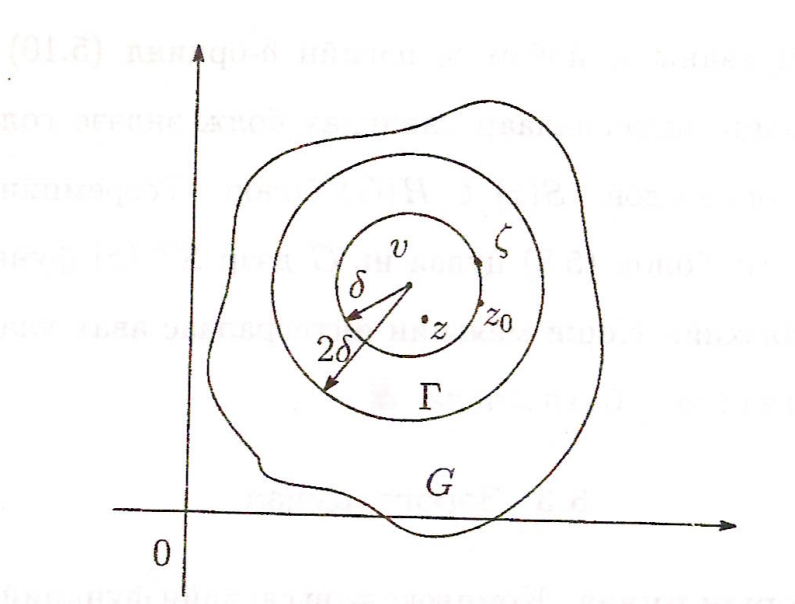
\includegraphics[width=6cm]{Zurag/17.PNG}
    \captionof{figure}{}
        \label{z.17}
\end{center}

$\zeta \in \Gamma=|z-z_0|=\delta$ байг. (\ref{5.5}) цувааны $z$-ийг $\zeta$-аар сольж $\dfrac{1}{2\pi i}\cdot \dfrac{1}{(\zeta - z)}$-аар үржүүлж авсан
\begin{eqnarray} \label{5.9}
   \dfrac{1}{2\pi i}\cdot \dfrac{S(\zeta)}{(\zeta -z)}=\dfrac{1}{2\pi i} \sum\limits_{k=1} ^\infty \dfrac{f_k(\zeta)}{\zeta -z}
\end{eqnarray}
цуваа сонирхъё.

(\ref{5.5}) цуваа $|z-z_0|=\delta$ тойрог дээр жигд нийлэх тул түүнийг гишүүнчлэн интегралчилж болно. Кошийн интеграл теорем ёсоор (\ref{5.9}) цувааны гишүүн бүрээс авсан интеграл нь $f_k(z)$-тэй тэнцэх тул
\begin{eqnarray} \label{5.10}
   \dfrac{1}{2\pi i} \int\limits_{\Gamma} \dfrac{S(\zeta)}{(\zeta -z)}d\zeta= \sum\limits_{k=1} ^\infty f_k(z)=\rho (z)
\end{eqnarray}
болно. 

(\ref{5.5})	цувааны нийлбэр $z_0$ цэгийн $\delta$-орчинд (\ref{5.10}) байдлаар Кошийн интегралаар тавигдах болж эндээс голоморф байх нь тогтоогдов. $S(z)\in H(G)$ болов. Теоремын хоёрдугаар хэсэг болох (\ref{5.8}) цуваа нь $G$ дээр $S^{(n)}(z)$ функц рүү жигд нийлэхийн Коши маягийн интегралаас авах уламжлалын томьёо ёсоор батлагдана. 
 \end{prf}
\section{Зэрэгт цуваа}
\textbf{1. Тейлорын цуваа.} Комплекс хувьсагчийн функцийн онолд зэрэгт цуваа онцгой үүрэг гүйцэтгэнэ.
\begin{eqnarray} \label{5.11}
   \sum\limits_{n=0}^\infty c_n(z-z_0)^n
\end{eqnarray}
дүрсийн цувааг зэрэгт цуваа \index{Зэрэгт цуваа} гэнэ.

$c_0, c_1, \ldots ,c_n,\ldots$ тогтмол комплекс тоонууд, $z_0$ бэхэлсэн тоо, $z$-комплекс хувьсах хэмжигдэхүүн. (\ref{5.11}) цуваа нь функцэн (\ref{5.5}) цувааны тухайн тохиолдол дээр нь (\ref{5.11}) цуваа нийлж байх бүх $z$-цэгүүдийн олонлогийг уул цувааны нийлэлтийн муж гэнэ. (\ref{5.11}) дүрсийн аливаа цуваа $z=z_0$ цэг дээр нийлэх нь илэрхий.

Зэрэгт цувааны үндсэн ухагдахуунуудын нэг болох дараах теорем авч үзье.
\begin{thm}
(Тейлор) \index{Тейлорийн теорем}. $f(z)\in H(D)$ бол энэ функц дурын \\ $U=\{z:|z-z_0|<R\}\subset D$ дугуй дээр нийлэх зэрэгт цувааны нийлбэр 
$$f(z)=\sum\limits_{n=0}^\infty c_n(z-z_0)$$
дүрстэй тавигдана.
\end{thm}
\begin{prf} 
$z\in U$ нь $z_0$-оос ялгаатай дурын цэг, $r$ тоог \\ $|z-z_0|<r<R$ байхаар сонгон авъя. $\{\zeta:|\zeta -z_0|=r\}$ тойргийг $\gamma$-ээр тэмдэглэе (зураг 18). Кошийн интеграл томьёо ёсоор
\begin{center}
    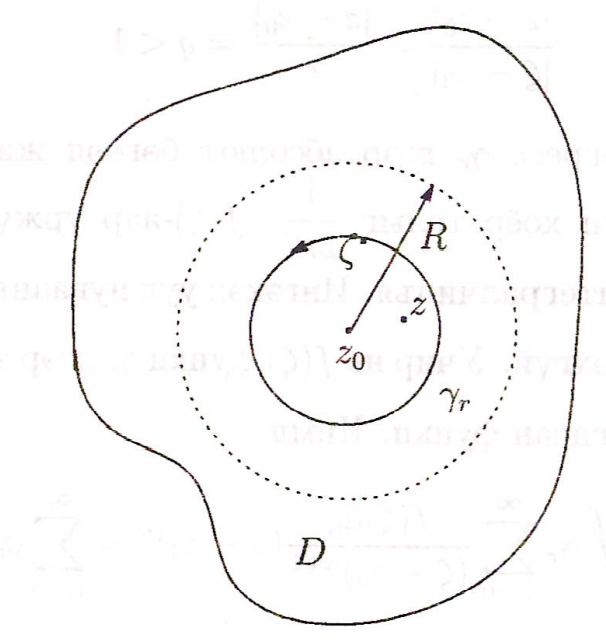
\includegraphics[width=5cm]{Zurag/18.PNG}
    \captionof{figure}{}
        \label{}
\end{center}
\begin{eqnarray}
    f(z)=\frac{1}{2\pi i}\int\limits_{\gamma_r}\frac{f(\zeta)d\zeta}{\zeta -z}
\end{eqnarray}
бөгөөд энэ функцийг цуваанд задлахын тулд $\dfrac{1}{\zeta -z}$ үржигдэхүүнийг $z-z_0$-ийн зэргээр геометр прогресс байдалтай тавих хэрэгтэй:
\begin{eqnarray} \label{5.13}
    \frac{1}{\zeta -z}=\frac{1}{(\zeta -z_0)\left(1-\frac{z-z_0}{\zeta -z_0}\right)}=\sum\limits_{n=0}^\infty \frac{(z-z_0)^n}{(\zeta -z_0)^{n+1}}
\end{eqnarray}
$\zeta \in \gamma_r$ байх бүхий л $\zeta$-ийн хувьд
$$\frac{|z-z_0|}{|\zeta -z_0|}=\frac{|z-z_0|}{r}=q<1$$
тул (\ref{5.13}) прогресс $\gamma_r$ дээр абсолют бөгөөд жигд нийлнэ. Одоо (\ref{5.13})-ийн хоёр талыг $\dfrac{1}{2\pi i}\cdot f(\zeta)$-аар үржүүлж $\gamma_r$-ээр гишүүнчлэн интегралчилъя. Ингэхэд уул цувааны жигд нийлэлтэд нөлөөлөхгүй. Учир нь $f(\zeta)$ функц $\gamma_r$ дээр тасралтгүй, улмаар зааглагдсан функц. Иймд
$$f(z)=\frac{1}{2\pi i}\int \gamma_r \sum\limits_{n=0}^\infty \frac{f(\zeta) d\zeta}{(\zeta -z_0)^{n+1}}(z-z_0)^n=\sum\limits_{n=0}^\infty c_n (z-z_0)^n$$
энд 
\begin{eqnarray} \label{5.14}
    c_n=\dfrac{1}{2\pi i} \int\limits_{\gamma_r} \frac{f(\zeta) d\zeta}{(\zeta -z_0)^{n+1}}, \quad n=0,1, \ldots
\end{eqnarray}
 \end{prf}
\begin{dfn}
 Коэффициент нь (\ref{5.14}) томьёонуудаар илэрхийлэгдэх (\ref{5.11}) цувааг $z_0$ төвт дугуй дээрх $f(z)$ функцийн Тейлорын цуваа \index{Тейлорын цуваа} гэнэ.
\end{dfn}
\begin{cor}
\textbf{(Кошийн тэнцэтгэл биш). } \index{Кошийн тэнцэтгэл биш}
$f(z)$ функц битүү $\overline{U}=\{|z-z_0|\leq r\}$ дугуй дээр голоморф. Мөн $\gamma_r =\partial U$ тойрог дээр түүний модуль $M$-ээс үл хэтрэх байг. Тэгвэл $z_0$ төвт дугуй дээрх Тейлорын цувааны коэффициентууд 
\begin{eqnarray}
    |c_n|\leq \frac{M}{r^{n}}, \quad (n=0,1,\cdots)
\end{eqnarray}
тэнцэл бишийг хангана.
\end{cor}
\begin{prf}
$\forall \zeta \in \gamma$ дээр $|f(\zeta)| \leq M$ байхыг тооцон (\ref{5.14}) томьёоноос олбол
$$|c_n|\leq \frac{1}{2\pi}\cdot \frac{M}{r^{n+1}}\cdot 2\pi r =\frac{M}{r^n}$$
 \end{prf}
Кошийн тэнцэл биш ашиглаж дараах сонирхолтой теорем батлагдана.
\begin{thm}
\textbf{(Лиувилль).} \index{Лиувиллийн теорем} $|f(z)|\leq M$ ба $f(z)\in H(\mathbb{C})$, $(\forall z\in \mathbb{C})$ байвал $f(z)=const $ байна. 
\end{thm}
\begin{prf}
Тейлорын теорем ёсоор $\overline{ U}=\{|z|\leq R\}$, $R<\infty$ дугуй дээр $f(z)$ функц Тейлорын цуваанд задрах тул \\ $f(z)=\sum\limits_{n=0}^\infty c_n z^n$ бөгөөд үүний коэффициентууд нь $R$-ээс үл хамаарах, нөгөө талаар $f(z$) нь $\mathbb{C}$ дээр зааглагдсан учир Кошийн тэнцэл биш ёсоор аливаа $n=0,1,\ldots$-ийн хувьд $|c_n|\leq \dfrac{M}{R^n}$.
Сүүлчийн тэнцэл бишийн баруун гар тал $n=1,2,\ldots$ үед \\ $R\rightarrow \infty$ байхад тэг рүү тэмүүлнэ. Харин зүүн гар тал $R$-ээс үл хамаарах, иймд $n=1,2,\ldots$ үед $c_n=0$ болж улмаар $f(z)=c_0.$
 \end{prf}

Лиувиллийн энэ теоремыг өргөтгөн томьёолж болно:
\begin{thm}
$f(z)\in H(\overline{\mathbb{C}})$ бол $f=const$ байна.
\end{thm}
\begin{prf}
$f(z)\in H(\infty)$ тул $\lim\limits_{z\rightarrow \infty} f(z)$ оршин байх ба төгсгөлтэй. Энд $f(z)$ нь $\infty$-ийн зааглагдсан олонлог дээр тасралтгүй байх функц хавтгай үлдсэн $\{|z|>R\}$ хэсэг дээр зааглагдсан нь илэрхий тул өмнөх теорем ёсоор $f(z)=const$
 \end{prf}
\begin{thm}
Абелийн теорем.\index{Абелийн теорем} Лемм.Хэрэв зэрэгт (\ref{5.11}) 
$$\sum\limits_{n=0}^\infty c_n(z-a)^n$$
цувааны гишүүд ямар нэг $z_0$ цэг дээр зааглагдсан, өөрөөр хэлбэл
\begin{equation} \label{5.16}
    |c_n (z_0-a)|\leq M, \quad n=0,1, \ldots
\end{equation}
байвал энэ цуваа $U=\{z:|z-a|<|z_0-a|\}$ дугуй дээр нийлэх ба компакт дэд олонлог $K\Subset U$ бүр дээр абсолют бөгөөд жигд нийлнэ.
\begin{center}
    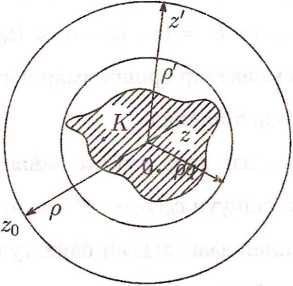
\includegraphics[width=4cm]{Zurag/19.jpg}
    \captionof{figure}{}
        \label{}
\end{center}
\end{thm}
\begin{prf}
$a\neq z_0$ байхаар $z_0$ авбал $|z_0-a|=\rho >0$. Ийм байхгүй бол $U$ хоосон олонлог.

$K\Subset U$ байг. Тэгвэл $\forall z\in K$ авахад $\dfrac{|z-a|}{\rho}\leq < 1$ (зураг 9) бөгөөд дурын $n=0,1, \ldots$ тооны хувьд
$$|c_n(z-a)^n|\leq |c_n|\cdot \rho^nq^n$$
байна. (\ref{5.16}) нөхцөлөөр $|c_n|\rho ^n\leq M$ болж $\forall z\in K$-ийн хувьд (\ref{5.11}) цуваа нийлэх геометр $M\sum\limits_{n=0}^\infty q^n$ прогрессоор мажорантлагдах тул тэр нь $K$ дээр абсолют бөгөөд жигд нийлнэ. Ингээд леммийн сүүлчийн өгүүлбэр батлагдав. Эхнийх нь эндээс мөрдөгдөн гарна. Учир нь $\forall z'\in U$ авахад тэр нь ямар нэг $|z'-a|<\rho '$ дугуйд оршино. $\rho '<\rho$ тул энэхүү шинэ дугуй нь $U$-д компактаар оршин байна. 
 \end{prf}
\begin{thm}
\textbf{(Абель). } Хэрэв зэрэгт (\ref{5.11}) цуваа $z_0\in \mathbb{C}$ цэг дээр нийлж байвал тэр нь $U=\{z:|z-a|< |z_0-a|\}$ дугуй дээр нийлэх ба $U$-д компактаар орших ямар нэг дэд олонлог дээр абсолют бөгөөд жигд нийлнэ.
\end{thm}
\begin{prf}
(\ref{5.11}) цуваа $z_0$ цэг дээр нийлж байвал харгалзах тоон цувааны ерөнхий гишүүн $c_n(z_0-a)^n$ тэг рүү тэмүүлнэ. Аливаа нийлэх дараалал зааглагдсан байх тул леммийн нөхцөл биелэгдэж теорем батлагдав. 
 \end{prf}
\begin{thm}
\textbf{Коши-Адамарын томьёо. } \index{Коши-Адамарын томьёо} Зэрэгт (\ref{5.11}) цуваа өгөгдсөн байг. $\overline{\lim\limits_{n\rightarrow \infty}} \sqrt{ |c_n|}= \wedge$ байвал $\wedge =0$ үед (\ref{5.11}) цуваа бүх хавтгай дээр абсолют нийлнэ.

$\wedge =\infty$ үед тэр нь зөвхөн $z=z_0$ цэг дээр нийлнэ. $z\neq z_0$ дээр сарнина.

$0<\wedge <\infty$ үед уул цуваа $|z-z_0|<\dfrac{1}{\wedge}$ дугуй дээр абсолют нийлэх ба энэ дугуйн гадна $\left(|z-z_0|>\dfrac{1}{\wedge}\right)$ сарнина.
\end{thm}
\begin{prf}
Зэрэгт (\ref{5.11}) цуваа $z_0$ дээр нийлэх тул энэ цувааны абсолют нийлэлтийг $z\neq z_0$ цэг дээр Кошийн шинж ашиглан
шинжилье.
\begin{eqnarray} \label{5.12}
    \sum\limits_{n=0}^\infty |c_n|\cdot |z-z_0|^n
\end{eqnarray} цуваа авъя. 
\begin{enumerate}
    \item [a)] $\wedge = 0$ гэвэл
    $$\overline{\lim} \sqrt[n]{|c_n||z-z_0|^n}=|z-z_0|\overline{\lim}\sqrt[n]{|c_n|}=0$$
    болж Кошийн шинжээр бүх хавтгай дээр (\ref{5.11}) цувааны абсолют нийлэлт тогтоогдлоо.
    \item [б)] $\wedge =\infty$ байг. $z\neq z_0$ байх аливаа $z$-ийн хувьд
    $$|z-z_0|\overline{\lim}\sqrt[n]{|c_n|}=\infty$$
    болж, өөрөөр хэлбэл (\ref{5.12}) цувааны ерөнхий гишүүн тэг рүү үл тэмүүлэх нь илэрхий тул (\ref{5.11}) цуваа $ z\neq z_0$ байх бүх цэг дээр сарнина.
    \item [в)] Эцэст нь $0<\wedge <\infty$ гэе. $z$ бүхний хувьд:
    $$\overline{\lim}\sqrt[n]{|c_n||z-z_0|^n}=|z-z_0|\cdot \wedge$$
Хэрэв $|z-z_0|<\dfrac{1}{\wedge}$ байвал $\overline{\lim}\sqrt[n]{|c_n||z-z_0|^n}<1$ болж (\ref{5.12}) цуваа Кошийн шинж ёсоор нийлнэ. \\ Иймд $|z-z_0|<\dfrac{1}{\wedge}$ дугуй дээр (\ref{5.11}) цуваа абсолют нийлнэ. Харин $|z-z_0|>\dfrac{1}{\wedge}$ үед $\overline{\lim\limits_{n\rightarrow\infty}}\sqrt[n]{|c_n||z-z_0|^n}>1$ болж (\ref{5.12}) цувааны ерөнхий гишүүн
тэг рүү үл тэмүүлэх учир улмаар (\ref{5.11}) цуваа $|z-z_0|>\dfrac{1}{\wedge}$ үед сарних нь тогтоогдов. 
\end{enumerate}
 \end{prf}
\begin{hnt}
\begin{eqnarray} \label{5.18}
    R=\frac{1}{\wedge}, \quad \wedge =\overline{\lim\limits_{n\rightarrow \infty}} \sqrt[n]{|c_n|}
\end{eqnarray}
шүтэлцлийг Коши-Адамарын томьёо гэнэ.
\end{hnt}
\begin{dfn}
 Зэрэгт (\ref{5.11}) цуваа нийлэх $z\in \mathbb{C}$ цэгүүдийн $E$ олонлог дахь задгай $\mathring{E}$ цөм (дотоод цэгүүдийн бөөгнөрөл)-ийг энэ цувааны нийлэлтийн муж гэнэ.
\end{dfn}
\begin{thm}
Зэрэгт (\ref{5.11}) цувааны нийлэлтийн муж нь \\ $|z-z_0|<R$ дугуй байна. $R$ тоо нь (\ref{5.18}) томьёогоор тодорхойлогдоно.
\end{thm}
\begin{prf}
Өмнөх тодорхойлолтоос харахад зэрэгт (\ref{5.11}) цувааны нийлэх цэгүүдийн $E$ олонлог $\{|z-z_0|=R\}$ тойргийн зарим цэгүүдээр сэлбэгдсэн $\{|z-z_0|<R\}$ дугуй байх учиртай. Иймд задгай $\mathring{E}$ цөм нь $|z-z_0|<R$ болой. 
 \end{prf}
Оршин байх нь саяны теоремоор нотлогдсон (задгай) дугуйг (\ref{5.11}) цувааны нийлэлтийн дугуй гэх ба $R$ тоог нийлэлтийн радиус гэнэ.
\begin{exm}
Дараах зэрэгт цуваануудын нийлэлтийн радиус ол.
\colhoy{
\begin{enumerate}
    \item [a)] $\displaystyle\sum\limits_{n=1}^\infty \dfrac{n!}{n^n}z^n$;
    \item [б)] $\displaystyle\sum\limits_{n=0}^\infty (3+(-1)^n)^nz^n;$
    \item [в)] $\displaystyle\sum\limits_{n=0}^\infty z^{2^n}$
\end{enumerate}
} 
\end{exm}
\begin{sol}
\begin{enumerate}
    \item  [a)] $$R=\lim\limits_{n\rightarrow \infty} \frac{n!}{n^n}\cdot \frac{(n+1)^{n+1}}{(n+1)!}=\lim\limits_{n\rightarrow \infty} \left(1+\frac{1}{n}\right)^n =e.$$
    \item [б)] $R=\overline{\lim\limits_{n\rightarrow \infty}}\sqrt[n]{\frac{1}{(3+(-1)^n)^n}}=\lim\limits_{n\rightarrow \infty} \sqrt[2k]{[3+(-1)^{2k}]^{2k}}=\dfrac{1}{4}.$
    \item [в)] Цувааг $\sum\limits_{k=0}^\infty a_kz^k$ дүрстэй бичиж болох ба үүнд 
    
    $a_k= \begin{cases}
     1, \quad \text{хэрэв} \quad k=2^n, \\
      0, \quad \text{хэрэв} \quad k\neq 2^n
    \end{cases}$ Иймд $R=\dfrac{1}{\overline{\lim\limits_{k\rightarrow \infty}}\sqrt[k]{|a_k|}}=1$
\end{enumerate}
\end{sol}
\begin{exm}

Дараах цуваануудыг нийлэлтийн дугуйн хил дээр шинжил.
\colgur{
\begin{enumerate}
    \item [a)] $\sum\limits_{n=1}^\infty \dfrac{(-1)^n}{n}z^n$;
    \item [б)] $\sum\limits_{n=0}^\infty \dfrac{n^2+1}{(z-i)^n}z^n;$
    \item [в)] $\sum\limits_{n=1}^\infty \dfrac{z^n}{n}.$
\end{enumerate}}
    
\end{exm}
\begin{sol}
\begin{enumerate}
    \item  [a)] $\wedge =1$, $R=1$. $|z|=1$ тойргийн $z=-1$-ээс ялгаатай цэг бүр дээр абсолют бишээр нийлнэ. 
    \item [б)] $\wedge =1$, $R=1$. $|z-i|=1$ тойрог дээр абсолют хэмжигдэхүүний цуваа $\sum\limits_{n=0}^\infty \dfrac{1}{n^2+1}$-нийлэх тул уул цуваа $|z-i|\leq 1$ гэсэн битүү дугуй дээр абсолют нийлнэ.
    \item [в)] $\wedge =1$, $R=1$. $|z|=1$  тойрог дээр цувааны нийлэлт шинжилье. Абсолют хэмжигдэхүүний  $\sum\limits_{n=1}^\infty \dfrac{1}{n}$ цуваа $|z|=1$ байх бүх цэг дээр сарнина. 
    
    $z\neq 1$, $|z|=1$ байхад $\sum\limits_{n=1}^\infty \dfrac{z^n}{n}$ цуваа нийлэхийг харуулъя. Дирихле-н шинж ашиглая. $b_n=\dfrac{1}{n}$, $a_n=z^n$, $|z|=1$ гэе. $b_n=\dfrac{1}{n}$ дараалал тэг рүү монотон тэмүүлнэ. Харин 
$$\left|\sum\limits_{k=1}^n z^k \right| = \left|\frac{z-z^{n+1}}{1-z}\right| <\frac{2}{|1-z|}, \quad z\neq 1$$ болж цувааны хэсгийн нийлбэрүүдийн дараалал зааглагдсан тул цуваа нийлнэ. 
\end{enumerate}
\end{sol}
\begin{thm}
\textbf{(Нийлбэрийн голоморф байх тухай). } Зэрэгт
\begin{eqnarray} \label{5.19}
    f(z)=\sum\limits_{n=0}^\infty c_n(z-a)^n 
\end{eqnarray} 
цувааны нийлбэр түүний нийлэлтийн дугуй дээр голоморф функц байна.
\end{thm}
\begin{prf}
$R>0$ гэе. Тэгэхгүй бол батлах зүйлгүй. (\ref{5.19}) цувааны хийсвэр уламжлал болох
\begin{eqnarray} \label{5.15}
    \sum\limits_{n=1}^\infty nc_n (z-a)^{n-1}=\varphi (z)
\end{eqnarray}
цувааны нийлэх буюу сарних нь $\sum\limits_{n=1}^\infty nc_n(z-a)^n$ цуваатай  адил. Учир нь
$$\overline{\lim\limits_{n\rightarrow \infty}} \sqrt[n-1]{n|c_n|} = \overline{\lim\limits_{n\rightarrow \infty}} (n|c_n|)^{\frac{1}{n}\cdot \frac{n}{n-1}} =\overline{\lim\limits_{n\rightarrow \infty}} \sqrt[n]{n|c_n|}.$$
Харин 
$$\overline{\lim\limits_{n\rightarrow \infty}} \sqrt[n]{n|c_n|} =\overline{\lim\limits_{n\rightarrow \infty}} \sqrt[n]{|c_n|}$$ байх тул (\ref{5.15}) цувааны нийлэлтийн радиус бас л $R$ байна. $U=\{|z-a|<R\}$ дугуйн компакт дэд олонлогууд дээр (\ref{5.15}) цуваа жигд нийлнэ. Иймд $\varphi (z)$ функц энэ дугуй дээр тасралтгүй. Мөн тийм шалтгаанаар (\ref{5.15}) цувааг $\Delta \Subset U$ байх дурын гурвалжны хилээр гишүүнчлэн интегралчилж болно:
$$\int\limits_{\partial \Delta} \varphi(z)dz=\sum\limits_{n=1}^\infty nc_n\int\limits_{\partial \Delta}(z-a)^{n-1}dz=0.$$
Баруун гар дахь бүх интеграл Кошийн теорем ёсоор тэгтэй тэнцүү, улмаар бас зүүн гар тал. Иймд, эх функц оршин байх тухай Теорем 5.13 ёсоор ашиглаж гаргах
$$\int\limits_{[a,z]} \varphi (\zeta)d\zeta=\sum\limits_{n=1}^\infty nc_n\int\limits_{[a,z]}(\zeta-a)^{n-1}d\zeta=\sum\limits_{n=1}^\infty c_n$$
функц (бид жигд нийлэлтийг дахин хэрэглэв) $z\in U$ цэг бүр дээр $\varphi(z)$-тэй тэнцэх уламжлалтай байна. Харин
$$f(z)=c_0+\int\limits_{[a,z]}\varphi (\zeta)d\zeta$$ 
$z\in U$ цэг бүр дээр уламжлалтай: $f'(z)=\varphi (z).$ 
 \end{prf}
\textbf{Голоморф функцийн чанарууд.} Зэрэгт цувааны нийлбэрийн голоморф байх тухай теоремын мөрдлөг байдлаар зарим теорем тэмдэглэе.
\begin{thm}
Аливаа $f(z)\in H(D)$ функцийн уламжлал $D$ дээр голоморф байна.
\end{thm}
\begin{prf}
$\forall z_0\in D$ дээр $U=\{|z-z_0|<R\}\subset D$ орчин байгуулъя. Тэгвэл Теорем 5.13 ёсоор $f'(z)=\varphi (z)$ уламжлал нь мөнхүү дугуй дээр нийлэх цуваа байдлаар тавигдана. Иймд $\varphi(z)$ дээр Теорем 5.13-ийг дахин хэрэглэвэл $\varphi(z)$ функц $U$ дээр комплекс анализын утгаар дифференциалчилагдах болов.
 \end{prf}
\begin{cor}
Тасралтгүй $f(z)$ функц $D$ дээр $F(z)$ хэмээх эх функцтэй байвал $f(z)\in H(D)$ байна. Теорем 5.14-ийг дахин хэрэглэж батлагдлаа.
\end{cor}
\begin{thm}
Аливаа $f(z)\in H(D)$ функц $D$ дээр бүхий л эрэмбийн уламжлалтай, тэдгээр нь $H(D)$ ангид харьяалагдана: $f^{(n)} (z)\in H(D)$.
\end{thm}
\begin{thm}
Хэрэв $f(z)$ функц $\{|z-z_0|<R\}$ дугуй дээр зэрэгт цувааны нийлбэр
\begin{eqnarray} \label{5.21}
    f(z)=\sum\limits_{n=0}^\infty c_n(z-z_0)^n
\end{eqnarray}
дүрсээр тавигдсан байвал энэ цувааны коэффициентууд
\begin{eqnarray} \label{5.22}
    c_n=\frac{f^{(n)}z_0}{n!}, \quad n=0,1,\ldots
\end{eqnarray}
томьёогоор нэгэн утгатай тодорхойлогдоно.
\end{thm}
\begin{prf}
(\ref{5.21}) тэнцэлд $z=z_0$ гэвэл $f(z_0)=c_0$ бөгөөд (\ref{5.21}) цувааг гишүүнчлэн дифференциалчилж $z=z_0$ гэвэл $f'(z_0)=c_1$ гэх мэтээр $f^{(n)}(z)=n!c_n+b_1(z-z_0)+\cdots $ болж $z=z_0$ гэвэл $f^{(n)}(z_0)=n!cn.$ 
 \end{prf}

Одоо (\ref{5.22}) томьёо ашиглан хялбар трансцендент $e^z$, $\sin z$, $\cos z$, $\sinh z$, $\cosh z$ функцүүдийн $z=0$ цэг дээрх зэрэгт цуваанд бичье:
\begin{eqnarray} \label{5.23}
    e^z=1+z+\frac{z^2}{2}+\cdots =\sum\limits_{n=0}^\infty \frac{z^n}{n!}, \quad R=\infty 
\end{eqnarray}
\begin{eqnarray} \label{5.24}
    \sin z=z-\frac{z^3}{3!}+\frac{z^5}{5!}-\cdots =\sum\limits_{n=0}^\infty (-1)^n\frac{z^{2n+1}}{(2n+1)!}, \quad R=\infty
\end{eqnarray}
\begin{eqnarray} \label{5.25}
    \cos z=1-\frac{z^2}{2!}+\frac{z^4}{4!}-\cdots =\sum\limits_{n=0}^\infty (-1)^n\frac{z^{2n}}{(2n)!}, \quad R=\infty
\end{eqnarray}
\begin{eqnarray} \label{5.26}
    \sinh z=z+\frac{z^3}{3!}+\frac{z^5}{5!}+\cdots =\sum\limits_{n=0}^\infty \frac{z^{2n+1}}{(2n+1)!}, \quad R=\infty
\end{eqnarray}
\begin{eqnarray} \label{5.27}
    \cosh z=1+\frac{z^2}{2!}+\frac{z^4}{4!}+\cdots =\sum\limits_{n=0}^\infty \frac{z^{2n}}{(2n)!}, \quad R=\infty
\end{eqnarray}
Энд (\ref{5.24})-ийг $i$-ээр үржүүлж (\ref{5.25}) дээр нэмэхэд Эйлерийн $e^{iz}=\cos z +i \sin z$ батлагдана. Хэрэв $f(z)$ функц $D$ муж дээр голоморф ба $G\Subset D$, $\forall z\in G$ байвал уламжлалын Кошийн томьёо 
\begin{eqnarray}
    f^{(n)}(z)=\frac{n!}{2\pi i}\int\limits_{\partial G}\frac{f(\zeta)d\zeta}{(\zeta -z)^{n+1}}, \quad n=0,1,2,\ldots
\end{eqnarray}
дүрстэй бичигдэнэ. Энэ томьёонууд Кошийн интеграл 
$$f(z)=\frac{1}{2\pi i}\int\limits_{\partial G} \frac{f(\zeta)d\zeta}{\zeta -z} $$
томьёоноос интеграл дор параметр $z$-ээр нь дифференциалчлах замаар гарна.
\begin{thm}
\textbf{(Морер).} \index{Морерийн теорем} Хэрэв $f(z)$ функц $D$ мужид тасралтгүй ба $$ \int\limits_{\partial \Delta}f(z)dz=0, \quad \forall \Delta \Subset D$$ байвал $f(z)\in H(D)$.
\end{thm}
\begin{prf}
$\forall a\in D$  цэгийн хувьд $U=\{|z-a|<r\}\subset D$ дугуй байгуулъя. $F(z)=\bint\limits_{[a,z]}f(\zeta) d\zeta$ функц $U$ дээр голоморф ба $z\in U$ цэг бүр дээр $F'(z)=f(z)$ тул өмнөх Теорем 5.14 ёсоор $f(z)\in H(D)$
 \end{prf}

Өгөгдсөн цэг дээр функцийн голоморф байхын өөр өөр тодорхойлолт хоорондоо чацуу чанартай.
\begin{thm}
Дараах гурван өгүүлбэр эквивалент:\\
$(R):f(z)$ функц $a$ цэгийн ямар нэг $U$ орчинд $\mathbb{C}$- дифференциалчлагдаж байвал $(C):f(z)$ функц $a$ цэгийн ямар нэг $U$ орчинд тасралтгүй ба $\bint\limits _{\partial \Delta}f(z)dz=0$, $\forall \Delta \Subset D$ байвал $(W):f(z)$ функц $a$ цэгийн ямар нэг $U$ орчинд нийлэх зэрэгт цуваанд задарч байвал энэ гурван өгүүлбэрийн аль нь ч биелэгдсэн $f(z)$ функц $a$ цэг дээр голоморф байна.\\
Эдгээр нотолгоо нь голоморф функцийн онолыг бүтээсэн гурван урсгалыг тусгана.

$(R)$ нөхцөлийг хангах функцийг Риманы утгаар голоморф \index{Риманы утгаар голоморф функц}, $(C)$ нөхцөлийг Кошийн утгаар голоморф \index{Кошийн утгаар голоморф функц}, $(W)$ нөхцөлийг Вейерштрассын утгаар голоморф \index{Вейерштрассын утгаар голоморф функц} байх функцүүд гэнэ.

$(R)\Rightarrow (C)$ нь Кошийн интеграл теоремоор, $(C)\Rightarrow (W)$ нь Тейлорын теоремоор. $(W)\Rightarrow (R)$ нь зэрэгт цувааны нийлбэрийн голоморф байх теоремоор тус тус батлагдана. 
\end{thm}
\begin{dfn}
 Дээр нь $f(z)$ функц тэг утга авах $\forall a\in\overline{\mathbb{C}}$ цэгийг, өөрөөр хэлбэл $f(z)=0$ тэгшитгэлийн язгуурыг уул \textbf{функцийн тэг} гэнэ.
\end{dfn}
\begin{thm}
Хэрэв $a$ цэг дээр голоморф бөгөөд тэр цэгийн ямар ч орчинд адилтган тэгтэй тэнцэхгүй $f(z)$ функцийн тэг нь $a$ байвал
\begin{eqnarray} \label{5.29}
     f(z)=(z-a)^n\varphi (z),
\end{eqnarray}
(энд $\varphi (z)$ функц нь $a$ цэг дээр голоморф, мөн түүнчлэн энэ цэгийн ямар нэг орчинд тэгээс ялгаатай утгатай байх функц) нөхцөлд тохирох натурал $n$ тоо оршин байна.
\end{thm}
\begin{prf}
$a$ цэгийн ямар нэг орчинд $f(z)$ функц зэрэгт цуваанд задарна. Сул гишүүн нь тэгтэй тэнцүү, учир нь $f(a)=0.$ Харин түүний бүх коэффициент тэгтэй тэнцэхгүй, хэрэв тэгвэл $f(z)=0$ байхад хүрнэ. Иймд тэгээс ялгаатай коэффициент олдох бөгөөд түүний хамгийн бага дугаарыг $n$-ээр тэмдэглэвэл задаргаа
\begin{eqnarray}
     f(z)=c_n(z-a)^n+c_{n+1}(z-a)^{n+1}+\cdots +c_n\neq 0
\end{eqnarray}
дүрстэй бичигдэнэ.


$a$ цэгийн ямар нэг орчинд нийлэх
$$c_n+c_{n+1}(z-a)+\cdots =\varphi (z)$$ цувааны нийлбэрийг $\varphi(z)$ гэж тэмдэглэвэл тэр нь энэ орчинд голоморф байна. $\varphi (a)=c_n\neq 0$ байх тул
$$f(z)=(z-a)^n\varphi (z)$$
нөхцөлд тохирох п дугаар оршин байна.
 \end{prf} 
\begin{thm}
\textbf{(Цор ганц байх тухай).} \index{Ганц ч чанарын теорем}\\
Хэрэв $f_1(z)$, $f_2(z)\in H(D)$ функцүүд $D$ мужид орших ядаж нэг хязгаарын $a$ цэгтэй $D$ олонлогт утгууд нь таарч байвал $D$ мужид газар сайгүй $f_1(z)=f_2(z)$ байна.
\end{thm}
\begin{prf}
$f(z)=f_1(z)-f_2(z)\in H(D)$ функц авъя. $D$ мужид $f(z)=0$ гэж батлах хэрэгтэй. Өөрөөр хэлбэл\\
$F=\{z\in D:f(z)=0\} \supset E$ олонлог $D$-тэй таарна. $f(z)$ функц тасралтгүй учраас хязгаарын $a$ цэг нь $f(z)$-ийн тэг байна. Теорем 5.14 ёсоор а-ийн ямар нэг орчинд $f(z)\equiv 0$. Тэгэхгүй бол энэ цэг $f(z)$-ийн тэгүүдийн олонлогийн хязгаарын цэг болж чадахгүй байна. Тийм учраас $F$ олонлогийн задгай $\mathring{F}$ цөм (өөрөөр хэлбэл түүний дотоод цэгүүдийн бөөгнөрөл) хоосон биш, тэр нь $a$ цэгийг агуулна. Байгуулалт
ёсоор  $\mathring{F}$  нь задгай, бас тэр нь битүү ($D$ мужийн харьцангуй топологит). Учир нь хэрэв $b\in D$ нь $\mathring{F}$ олонлогийн орчинд $b$ байх өөрөөр хэлбэл $b\in \mathring{F}$. $D$ нь мужийн тодорхойлолтоор холбоост байх тул I бүлэг 4. Теорем 2 ёсоор $\mathring{F}=D$. 
 \end{prf}
\begin{dfn}
$f(z)$ функцийн хувьд 
\begin{eqnarray}
     f(a)=\cdots =f^{(n-1)}(a)=0, \quad f^{(n)}(a)\neq 0(n  \geq 1)
\end{eqnarray}
байвал $a\in\mathbb{C}$ цэгийг түүний $n$-эрэмбийн тэг \index{Тэгийн эрэмбэ} гэнэ. Тейлорын цувааны коэффициент олох $c_n=\dfrac{f^{(n)}}{n!}$ томьёоноос харахад тэгийн эрэмбэ нь уул функцийн энэ цэг дээрх Тейлорын задаргааны коэффициентын тэгээс ялгаатай бага дугаартай таарна, өөрөөр хэлбэл теорем 5.14-ээр томьёолсон $n$ тоотой тэнцэнэ. Тэгтэй адилтган тэнцүү биш голоморф функц төгсгөлгүй эрэмбийн тэгтэй байж чадахгүйг цор ганц байх тухай теорем зааж байна.

Олон гишүүнтийн үлгэрээр хуваагдахын шинжийн тусламжтайгаар тэгийн эрэмбийг тодорхойлж болно. 
\end{dfn}
\begin{thm}
Голоморф $f(z)$ функцийн $a\in\overline{\mathbb{C}}$ тэгийн эрэмбэ нь $\dfrac{f(z)}{(z-a)^k}$ ноогдвор $a$ дээр голоморф байхуйц $(z-a)^k$ зэргийн  хамгийн их эрэмбэтэй таарна.
\end{thm}
\begin{prf}
$a$ тэгийн эрэмбийг $n$-ээр, $f(z)$-ийн хуваагдах $z-a$ биномын хамгийн их эрэмбийг $N$-ээр тус тус тэмдэглэе. (\ref{5.29}) томьёо ёсоор $f(z)$ аливаа $k\leq n$ зэрэгт хуваагдах тул
$$\frac{f(z)}{(z-a)^k}=(z-a)^{n-k}\varphi (z).$$
 \end{prf}
Иймд $N\geq n$. $f(z)$ функц $(z-a)^n$ зэрэгт хуваагдана гэе.
Өөрөөр хэлбэл
$$\frac{f(z)}{(z-a)^N}=\psi(z)$$
ноогдвор $a$ цэг дээр голоморф функц дүрсэлнэ. $\psi (z)$ функцийг $(z-a)$-ийн зэргээр цуваанд задлаад улмаар $f(z)$ функцийн $a$ цэг дээрх Тейлорын задаргаа $N$-ээс багагүй зэрэгтээр бичигдэх нь илэрхий. Иймд $N\leq n$ болж өмнөхтэй нэгтгэхэд $N=n$ байх нь тогтоогдов.
\begin{exm}
$f(z)=\dfrac{z^7}{1-\cos z}$ функцийн $z=0$ байх тэгийн эрэмбийг ол.
\end{exm}
\begin{sol}
$$f(z)=\frac{z^7}{1-\left(1-\frac{z^2}{2!}+\frac{z^4}{4!}-\cdots \right)}=\frac{z^5}{\frac{1}{2!}-\frac{z^2}{4!}+\cdots}=z^5\varphi(z),$$ энд $\varphi (z)=\dfrac{1}{\frac{1}{2}-\frac{z^2}{4}+\cdots}$ тул $\varphi (0)\neq 0$ болж (\ref{5.29}) томьёо ёсоор $z=0$ нь 5-р эрэмбийн тэг юм. Энэ бодлогыг 
$$\left(\frac{z^7}{1-\cos z}\right)^{(v)}\neq 0$$
байхаар ч шийдэж болно. 
\end{sol}
\begin{hnt}
$f(z)$ функц $\infty$ дээр голоморф бөгөөд $\infty$ нь түүний тэг байг. Энэ $\infty$ хэмээх тэгийн эрэмбэ нь $\varphi (z)=f\left(\dfrac{1}{z}\right)$ функцийн $a=\infty$ гэсэн тэг цэгийн эрэмбэ гэдэг нь ойлгомжтой. $a=\infty$ цэгийн хувьд өмнөх теорем хүчинтэй, харин $(x-a)^k$-д хуваахын оронд $z^k(k=1,2,\ldots)$-аар үржүүлж авна.

Функцийн тэг цэгийн эрэмбийн ухагдахууныг голоморф функцийн $A$-цэгийнх болгон өргөтгөж болно.

$a\in\overline{\mathbb{C}}$ цэгийн хувьд $f(a)=A$ байвал түүнийг $f(z)$ функцийн $A$ цэг \index{A-цэг} гэнэ. $a$ дээр голоморф $f(z)$ функцийн $A$-цэгийн эрэмбэ \index{A-цэгийн эрэмбэ} нь $f(z)-A$ функцийн тэг цэгийн эрэмбэ байна.
\end{hnt}
\begin{thm}
\textbf{(Вейерштрасс).}  $f(z)\in H(D)$ функцүүдийн
\begin{eqnarray} \label{5.32}
     f(z)=\sum\limits_{n=0}^\infty f_n(z)
\end{eqnarray} 
цуваа $\forall G\Subset D$ дээр жигд нийлж байвал
\begin{enumerate}
    \item $f(z)\in H(D)$
    \item Цувааг $\forall z\in D$ дээр гишүүнчлэн дифференциалчилагдана. 
\end{enumerate}
\end{thm}
\begin{prf}
$\forall a\in D$ байг. $U=\{z:|z-a|<r\}\Subset D$ дугуй авъя. (\ref{5.32}) цуваа өгөгдсөн нөхцөл ёсоор $U$ дээр жигд нийлэх ба гишүүд нь $U$ дээр тасралтгүй, улмаар $f(z)$ нь $U$ дээр тасралтгүй байна.

$\Delta \subset U$ авахад $\partial \Delta$ дээр (\ref{5.32}) цуваа жигд нийлэх тул түүнийг гишүүнчлэн интегралчилж болох тул
$$\int\limits_{\partial \Delta}f(z)dz=\sum\limits_{n=0}^\infty \int\limits_{\partial \Delta}f(z)dz=0$$
болж Морера-ийн теорем ёсоор $f(z)\in H(U)$ болж 1) нь батлагдав.

Одоо 2)-ийг батлахын тулд $a\in D$ цэгийн хувьд дахиад л $U=\{|z-a|<r\}\Subset D$ дугуй авъя. $|z-a|=r$ тойргийг $\partial U$ гэвэл уламжлалын Кошийн теорем ёсоор
\begin{eqnarray} \label{5.33}
     f^{(n)}(a)=\frac{n!}{2\pi i}\int\limits_{\partial U} \frac{f(z)dz}{(z-a)^{n+1}}, \quad n=0,1,\ldots
\end{eqnarray}
байна. 

$U$ дээр 
\begin{eqnarray} \label{5.34}
     \frac{f(z)dz}{(z-a)^{k+1}}=\sum\limits_{k=0}^\infty \frac{f_n(z)}{(z-a)^{k+1}}
\end{eqnarray}
(энэ нь (\ref{5.32})-аас $\forall \in\partial U$-ийн хувьд модуль нь $\dfrac{1}{r^{k+1}}$-тай тэнцэх үржигдэхүүнээр ялгагдана) цуваа жигд нийлэх учраас (\ref{5.34})-ийг (\ref{5.33}) интегралд тавьж болно:
$$f^{(k)}(a)= \sum\limits_{k=0}^\infty \frac{k!}{2\pi i} \int\limits_{\partial U} \frac{f_{n}(z)dz}{(z-a)^{k+1}}=\sum\limits_{k=0}^\infty f_n^{(k)}(a)$$ болж 2) батлагдав. 
 \end{prf}

Анализад олон гишүүнтээс зохиосон цуваа онцгой үүрэг гүйцэтгэдэг. Вейерштрассын теорем ёсоор хэрэв олон гишүүнтүүдийн 
\begin{eqnarray}
     f(z)=\sum\limits_{n=0}^\infty P_n(z)
\end{eqnarray}
цуваа ямар нэгэн $D$ мужид компактаар орших дэд олонлог бүр дээр жигд нийлж байвал түүний нийлбэр $f(z)\in H(D)$ гэж батлагдана.

Практикт, $f(z)\in H(D)$ байх аливаа функцэд олон гишүүнтүүдийн дарааллаар дөхөх урвуу бодлого чухал байдаг. Олон гишүүнтээр жигд дөхөх тухай бодлогын тавилттай танилцъя:\\
$D\subset \overline{\mathbb{C}}$ муж болон $f(z)\in H(D)$ гэж өгөгдсөн байг.

Дурын $K\Subset D$ олонлог ба дурын $\varepsilon >0$ тооны хувьд
\begin{eqnarray}
     ||f(z)-P(z)||_k=\sup_{z\in K}|f(z)-P(z)|<\varepsilon
\end{eqnarray}
байхаар $P(z)$ олон гишүүнт байгуулах шаардлагатай. Энэ бодлого нь $D$ мужийн компакт дэд олонлог бүр дээр $f(z)$-рүү жигд нийлэх олон гишүүнтүүдийн $\sum\limits_{n=0}^\infty P_n(z)$ цуваа байгуулахтай чацуу чанартай бодлого юм.
\begin{exm}
$f(z)=(z^2-1)\sinh z$ функцийг $z_0=0$ цэг дээр цуваанд задал.
\end{exm} 
\begin{sol}
\ref{5.26} ёсоор 
\begin{align*}
    (z^2-1)\sinh z&=(z^2-1)\sum\limits_{n=0}^\infty \frac{z^{2n+1}}{(2n+1)!} \\
    &=\sum\limits_{n=0}^\infty \frac{z^{2n+3}}{(2n+1)!}-\sum\limits_{n=0}^\infty\dfrac{z^{2n+1}}{(2n+1)!}
\end{align*}
\end{sol}
\begin{exm}
$e^{-z^2}$ функцийг $z_0=0$ цэг дээр цуваанд задал.
\end{exm} 
\begin{sol}
(\ref{5.23}) задаргаанд $-z^2$-ийг $z$-ийн оронд тавьж
$$e^{-z^2}=1-z^2+\frac{z^4}{2!}+\cdots =\sum\limits_{n=0}^\infty (-1)^n\frac{z^{2n}}{n!}$$
\end{sol}
\begin{exm}
$\sin^2z$ функцийг $z_0=0$ цэг дээр цуваанд задал.
\end{exm}
\begin{sol}
$\sin^2 z=\dfrac{1}{2}-\dfrac{1}{2}\cos 2z$ тэнцэлд (\ref{5.25}) томьёо ашиглавал 
$$\sin^2 z=\sum\limits_{n=0}^\infty (-1)^{n+1}\frac{2^{2n-1}z^{2n}}{(2n)!}.$$
\end{sol}
\begin{exm}
$f(z)=\ln (1+z)$, $f(0)=1$ функцийг $z$-ийн зэргээр цуваанд задал.
\end{exm}
\begin{sol}
Геометрийн прогресс $\dfrac{1}{1+z}=\sum\limits_{n=0}^\infty (-1)^n z^n; \ \ |z|<1$ дугуй дээр нийлэх тул гишүүнчлэн интегралчилбал
\begin{align*}
    f(z)&=\ln (1+z)=\bint\limits_0^z \frac{dz}{1+z}=z-\frac{z^2}{2}+\frac{z^3}{3}-\cdots \\
    &=\sum\limits^{n=0}_\infty (-1)^n\frac{z^{n+1}}{n+1}, \quad R=1.
\end{align*}
\end{sol}
\begin{exm}
$\dfrac{z}{z+2}$ функцийг $z_0=1$ цэгийн орчинд өөрөөр хэлбэл $z-1$-ийн зэргээр цуваанд задал.
\end{exm}
\begin{sol}
$\dfrac{z}{z+2}=\dfrac{z-1+1}{3\left(1+\frac{z-1}{3}\right)}$ тул 
$$\frac{z}{z+2}\sum\limits _{n=0}^\infty \frac{(-1)^n}{3^{n+1}}(z-1)^{n+1} +\sum\limits_{n=0}^\infty \frac{(-1)^n}{3^{n+1}}(z-1)^n, \quad R=3.$$
\end{sol}
\begin{exm}
$\dfrac{1}{3-2z}$ функцийг $z_0=3$ цэг дээр цуваанд задалж, 
нийлэлтийн радиусыг ол.
\end{exm}
\begin{sol}
$$\frac{1}{3-2z}=\frac{1}{3-2(z-3+3)}=\frac{1}{-3-2(z-3)}=-\frac{1}{3}\frac{1}{1+\frac{2(z-3)}{3}}$$ бөгөөд 
$\left|\dfrac{2(z-3)}{3}\right| <1$, өөрөөр хэлбэл $|z-3|<\dfrac{3}{2}$ үед 
$$\frac{1}{3-2z}=-\frac{1}{3}\sum\limits_{n=0}^\infty (-1)^n\left(\frac{2}{3}\right)^n (z-3)^n=\sum\limits_{n=0}^\infty \frac{(-1)^{n+1}2^n}{3^{n+1}}(z-3)^n, $$
$$R=\frac{3}{2}.$$
\end{sol}
\begin{exm}
$\dfrac{1}{1-z+z^2}$ функцийг $z$-ийн зэргээр задал.
\end{exm}
\begin{sol}
\begin{align*}
  \dfrac{1}{1-z+z^2}&=\dfrac{1+z}{1+z^3} \\
  &=\sum\limits_{n=0}^\infty (-1)^n z^{3n}+\sum\limits_{n=0}^\infty (-1)^nz^{3n+1}, \quad R=1.  
\end{align*}
\end{sol}
\begin{center}
    \textbf{Дасгал}
\end{center}
\begin{enumerate}
    \item 
Дараах функцүүдийг $(z-z_0)$-ийн зэргээр Тейлорын цуваанд задал. Нийлэлтийн радиусыг ол.
\colhoy{
\begin{enumerate}
    \item [a)] $\cos 2z, z_0=1$
     \item [б)] $ze^{-z}, z_0=1$
      \item [в)] $\dfrac{1}{z-1}, z_0=2$
      \item [г)] $\dfrac{z}{z^2+4}, z_0=2$
       \item [д)] $\cos^2z, z_0=\pi$
        \item [е)] $\dfrac{z}{z^2-2z-3}, z_0=0$
         \item [ж)] $e^z, z_0=\dfrac{1}{2}$
          \item [з)] $\cos z, z_0=-\dfrac{\pi}{4}$
\end{enumerate}
}
\item Дараах функцүүдийн тэг цэг олж, тэдгээрийн эрэмбийг тогтоо.
\colgur{
\begin{enumerate}
    \item [a)] $1+\cos z$
    \item [б)] $z^4+4z^2$
    \item [в)] $z\sin z -z^2$
\end{enumerate}
}
\end{enumerate}